%=====================
%  RESULTS
%=====================

\begin{figure}[!tb]
	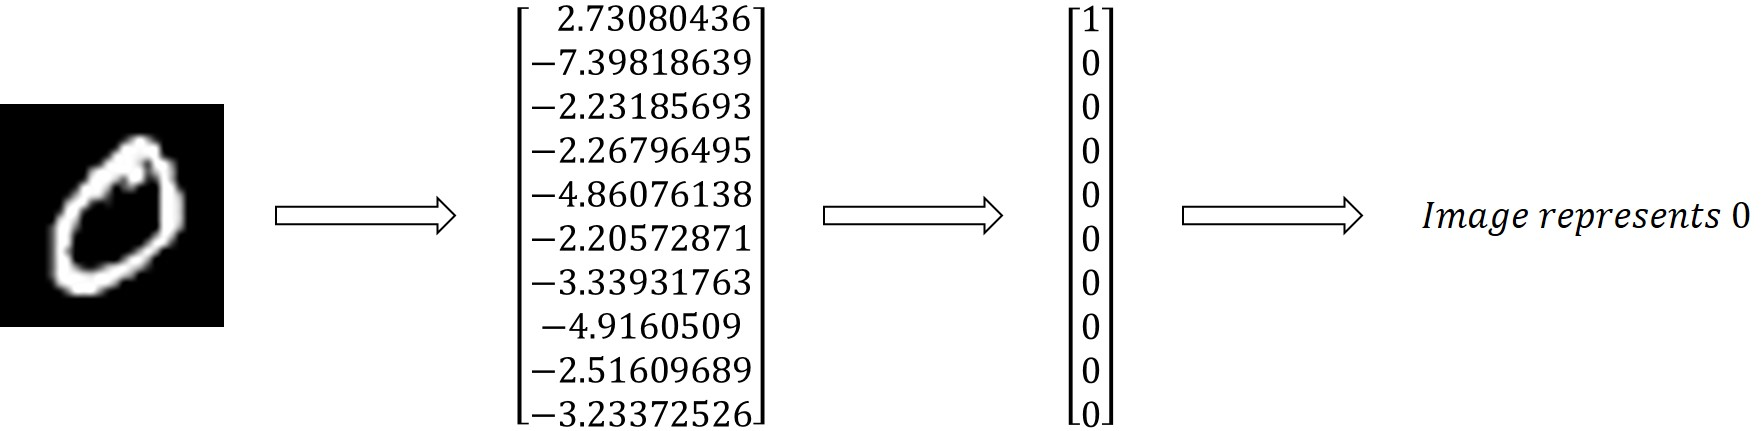
\includegraphics[width=15cm, height=4cm]{sample-workflow}
	\centering
	\caption{With the given image (pixel values), we compute the output with respect to each of the $10$ hyperplanes. The output is vectorized with $i$-th element of the vector representing the output with the hyperplane that distinguishes between digit $i-1$ and the rest. We then take all the values that yielded a positive output to determine which class the image belongs to.}
	\label{fig:workflow}
\end{figure}

With the techniques, and assumptions described in the previous section, we used Python and \texttt{sklearn} to build a Support Vector Machine classifier to classify handwritten digits from the MNIST dataset.

We first fit our hyperlanes using $60,000$ training images without any kernel transform i.e., we used the linear kernel. Then, we tested the accuracy of our hyperplanes by using it to classify $10,000$ testing images. With the linear kernel, we got an accuracy of $86.49 \%$. Figure \ref{fig:workflow} shows how we processed the output from each of the $10$ hyperplanes and then deciphered to which class the image belonged to. Some of the important code snippets are discussed in Appendix \ref{appendix:code}.

We then transformed our data with the polynomial kernel. We first used a quadratic transformation, and then a cubic transformation. We also tried using the sigmoid kernel\footnote{Sigmoid kernel uses the transformation $K(\vec{x}, \vec{y}) = \tanh(\gamma\vec{x}^{\text{T}}\vec{y} + r)$ where $\gamma$ and $r$ are the kernel parameters. We used $\gamma=\frac{1}{m}=\frac{1}{60,000}$ and $r=0$.}. Our results for all of these are summarized in Table \ref{tab:results}.

As we can see from Table \ref{tab:results}, our data (the images) is not completely linearly separable. In fact, we get the best accuracy on our testing images when we used a polynomial of degree $2$ i.e., a quadratic transformation. It makes sense to think that transforming the data into the wrong feature space will make it harder, and sometimes impossible, to find a decent hyperplane that separates the data. Our intuition is supported by the sigmoid kernel where our accuracy drops by a factor of $10$ compared to the linear kernel.

\begin{table*}[!tb]
	\centering
	\begin{tabular}{lcc}
		\toprule
		\multicolumn{3}{c}{\textbf{Accuracy of our classifiers}} \\
		\midrule
		Kernel & Training Accuracy & Testing Accuracy \\
		\midrule
		Linear & $87.27$ \% & $86.49$ \% \\
		Polynomial (deg=$2$) & $100$ \% & $98.08$ \% \\
		Polynomial (deg=$3$) & $99.99$ \% & $97.85$ \% \\
		Sigmoid & $9.92$ \% & $10.09$ \% \\
		\bottomrule
	\end{tabular}
	\caption{Accuracy of different classifiers}
	\label{tab:results}
\end{table*}